\chapter{Implementation and Testing}
\label{ch:testing}


\section{Third-party Modules in the Playbook}

The implementation requires two third-party modules for managing Keystone endpoints and services. Both modules have been created by Davide Guerri <davide.guerri@gmail.com>, licensed under Apache License, Version 2.0, and are included as part of the playbook.

\section{Testing of the Deployment}

I have prepared the following setup to for testing the environ
\subsection{Description of the Host Environment}

The reference testing environment consists of three virtual machines with the following specification:

\subsubsection*{Controller}

\begin{itemize}
  \item{CPUs: 2}
  \item{RAM: 2048 MB}
  \item{Disk: 30 GB}
\end{itemize}

\subsubsection*{Compute}

\begin{itemize}
  \item{CPUs: 4}
  \item{RAM: 6144 MB}
  \item{Disk: 30 GB}
\end{itemize}

\subsubsection*{Storage}

\begin{itemize}
  \item{CPUs: 1}
  \item{RAM: 1536 MB}
  \item{Disk1: 20 GB}
  \item{Disk2: 60 GB}
\end{itemize}

These virtual machines were running on a laptop with the following configuration:

\begin{itemize}
  \item{CPU: 2.8 GHz Intel i7 4980HQ}
  \item{RAM: 16 GB}
  \item{SSD: PCIe 3.0 x4 8.0 GT/s (25.6 Gbit/s)}
\end{itemize}

\subsection{Using Ansible with Vagrant}

Vagrant is a tool that manages virtual machines for development environment. It uses private key authentication and generates its own keys for the virtual machines.

First, Vagrant needs to be configured to use a single private key to authenticate to all three virtual machines. To achieve this, the following line needs to be put in the \texttt{Vagrantfile}:


\begin{lstlisting}
config.ssh.insert_key = false
\end{lstlisting}



Vagrant routes SSH ports of the guest virtual machines to the localhost and uses different port for each. A command \texttt{vagrant ssh-config} will show the ports of each virtual machine. These ports need to be used in the \texttt{hosts} file. An example might look like this:

\begin{lstlisting}
controller ansible_ssh_host=127.0.0.1 ansible_ssh_port=2222
compute1 ansible_ssh_host=127.0.0.1 ansible_ssh_port=2200
compute1 ansible_ssh_host=127.0.0.1 ansible_ssh_port=2201
\end{lstlisting}

The last step is to configure Ansible to use the correct user name and private key. This can be done by creating file called \texttt{ansible.cfg} with the following content:

\begin{lstlisting}
[defaults]
hostfile = hosts
remote_user = vagrant
private_key_file = ~/.vagrant.d/insecure_private_key
host_key_checking = False
\end{lstlisting}

\subsection{Running the Deployment}

To deploy the OpenStack cloud in the testing environment using the Ansible playbook, you need to provision the virtual machines and run the playbook. The virtual machines can be provisioned using Vagrant by issuing the following command:

\begin{lstlisting}
$ vagrant up
\end{lstlisting}

This will create three virtual machines matching the physical architecture. When the virtual machines are ready, you can run the Ansible playbook by issuing the following command:

\begin{lstlisting}
$ ansible-playbook deploy-openstack.yml
\end{lstlisting}

This will deploy the OpenStack cloud on the virtual machines created before. The playbook assumes that you have an internet connection available to all three virtual machines. When running the deployment, the installation took approximately 7 minutes.

\subsection{Testing the Deployment}

When the deployment is finished, I have tested the setup using the web interface which was available on \texttt{http://10.0.0.11/dashboard} when using the default configuration. The default login details are:

\begin{itemize}
  \item{Domain: \texttt{default}}
  \item{User: \texttt{admin}}
  \item{Password: \texttt{redhat}}
\end{itemize}

\subsubsection{Checking Running Services}

The dashboard shows the OpenStack services running in the environment (shown on picture \ref{fig:screenshot_services}), the compute services (shown on picture \ref{fig:screenshot_compute}), the block storage services (shown on picture \ref{fig:screenshot_storage}), and the network agents (shown on picture \ref{fig:screenshot_network}). This means that all the services are up and running.


\begin{figure}[!h]
  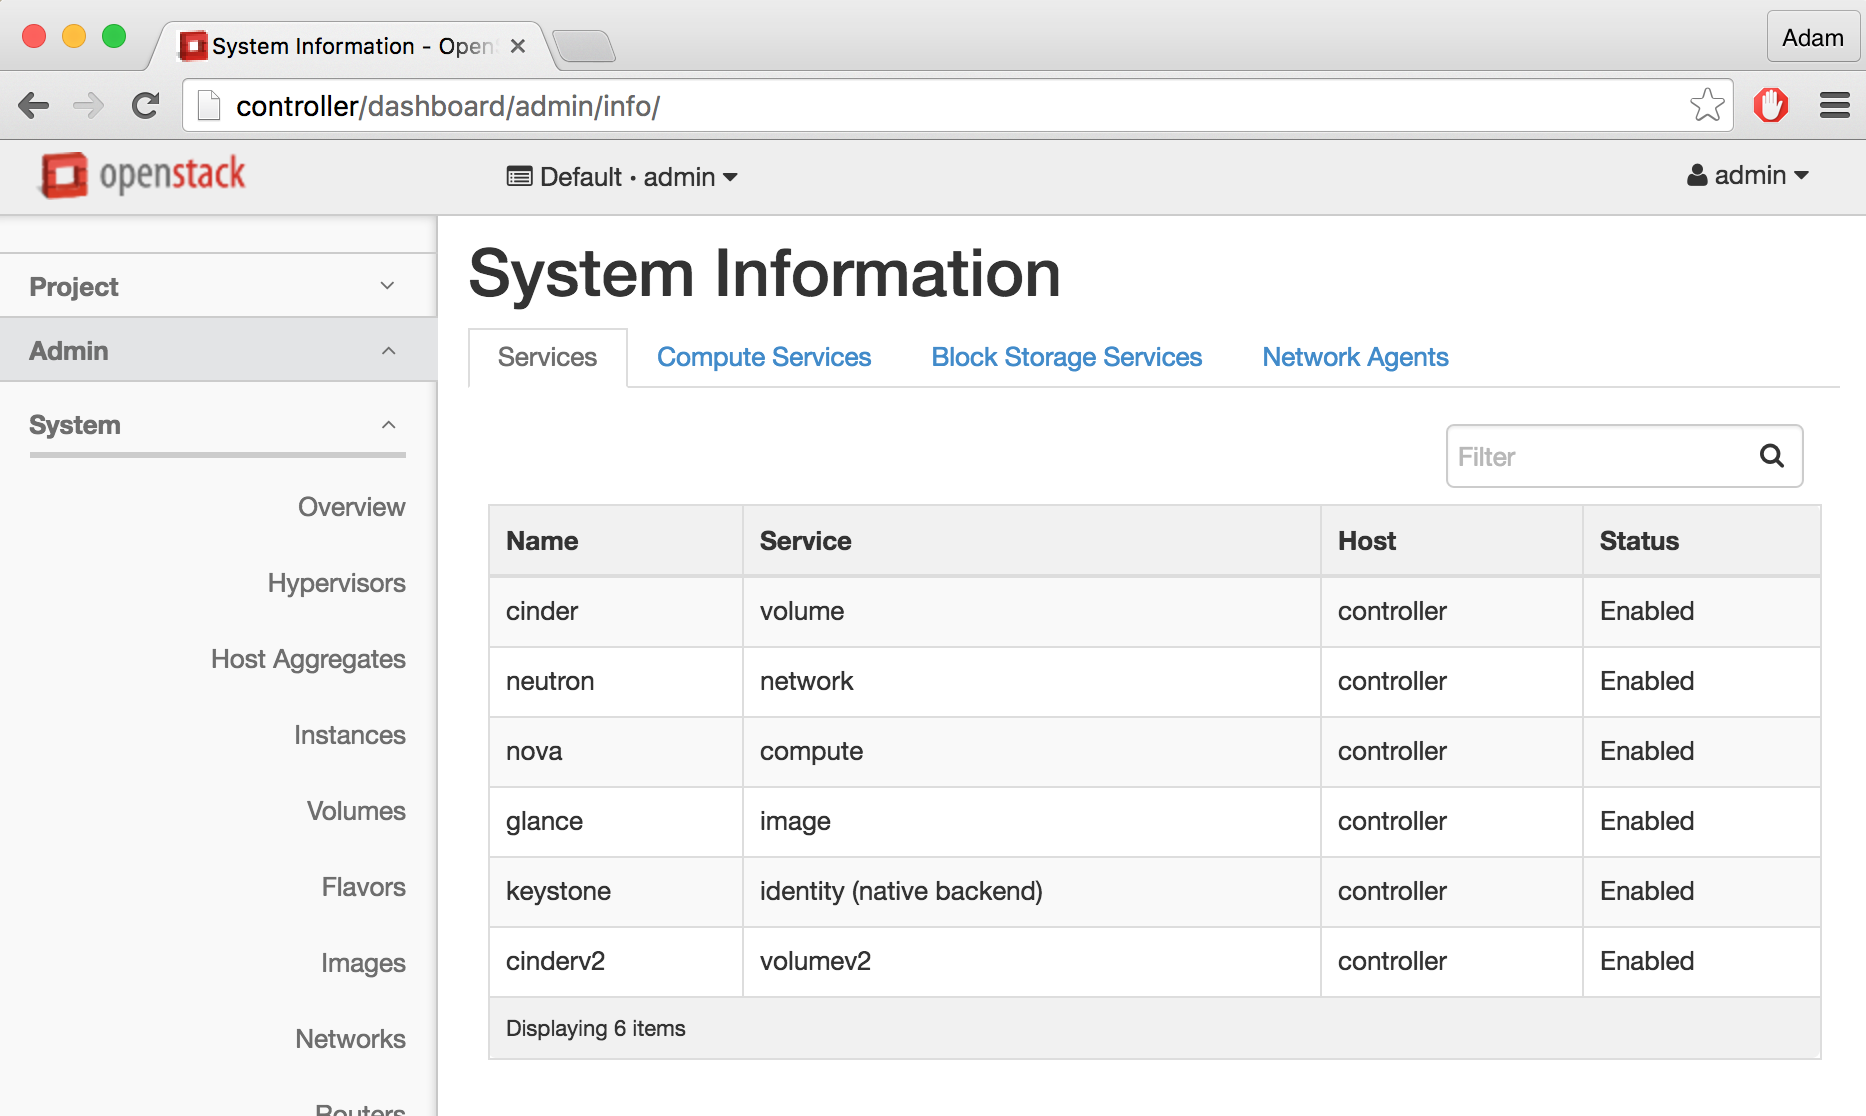
\includegraphics[width=\textwidth]{fig/screenshot_services.png}
  \caption{The OpenStack Dashboard shows the OpenStack services running}
  \label{fig:screenshot_services}
\end{figure}


\begin{figure}[!h]
  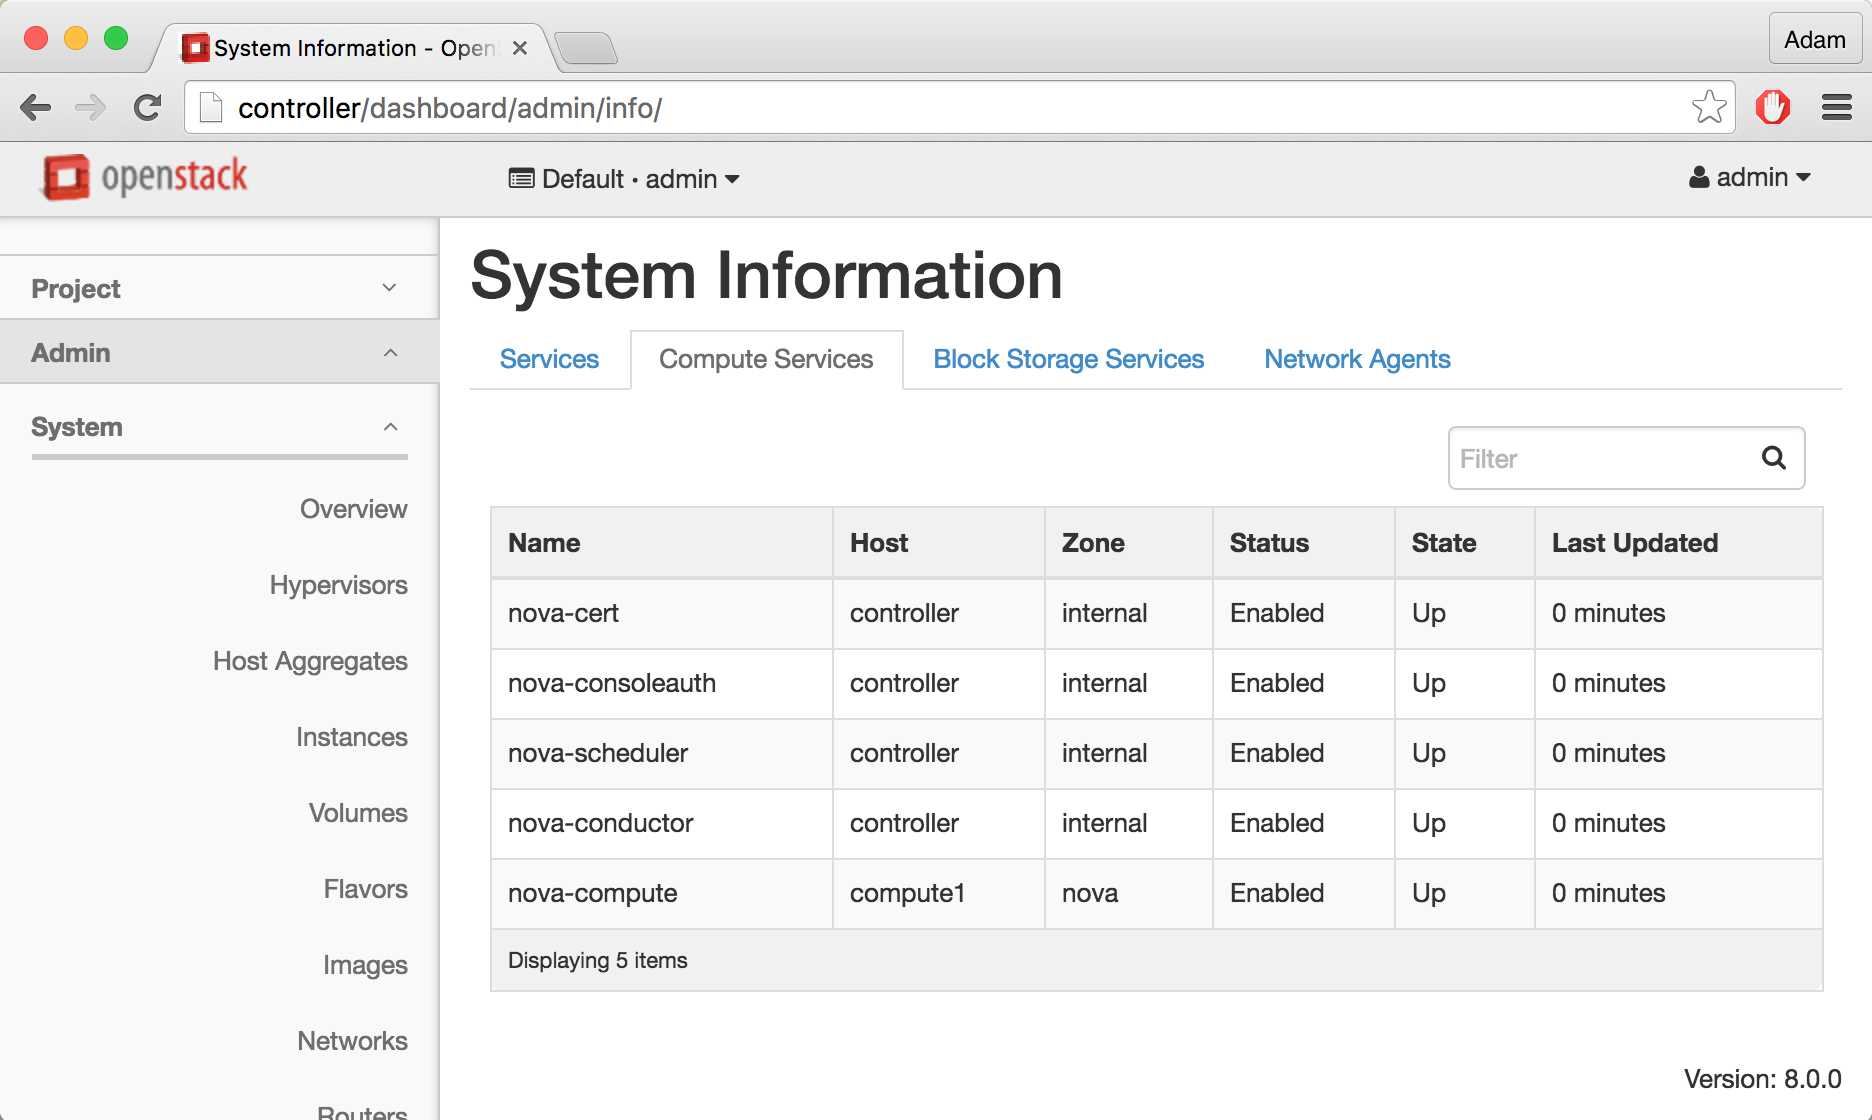
\includegraphics[width=\textwidth]{fig/screenshot_compute.png}
  \caption{The OpenStack Dashboard shows the compute services running}
  \label{fig:screenshot_compute}
\end{figure}


\begin{figure}[!h]
  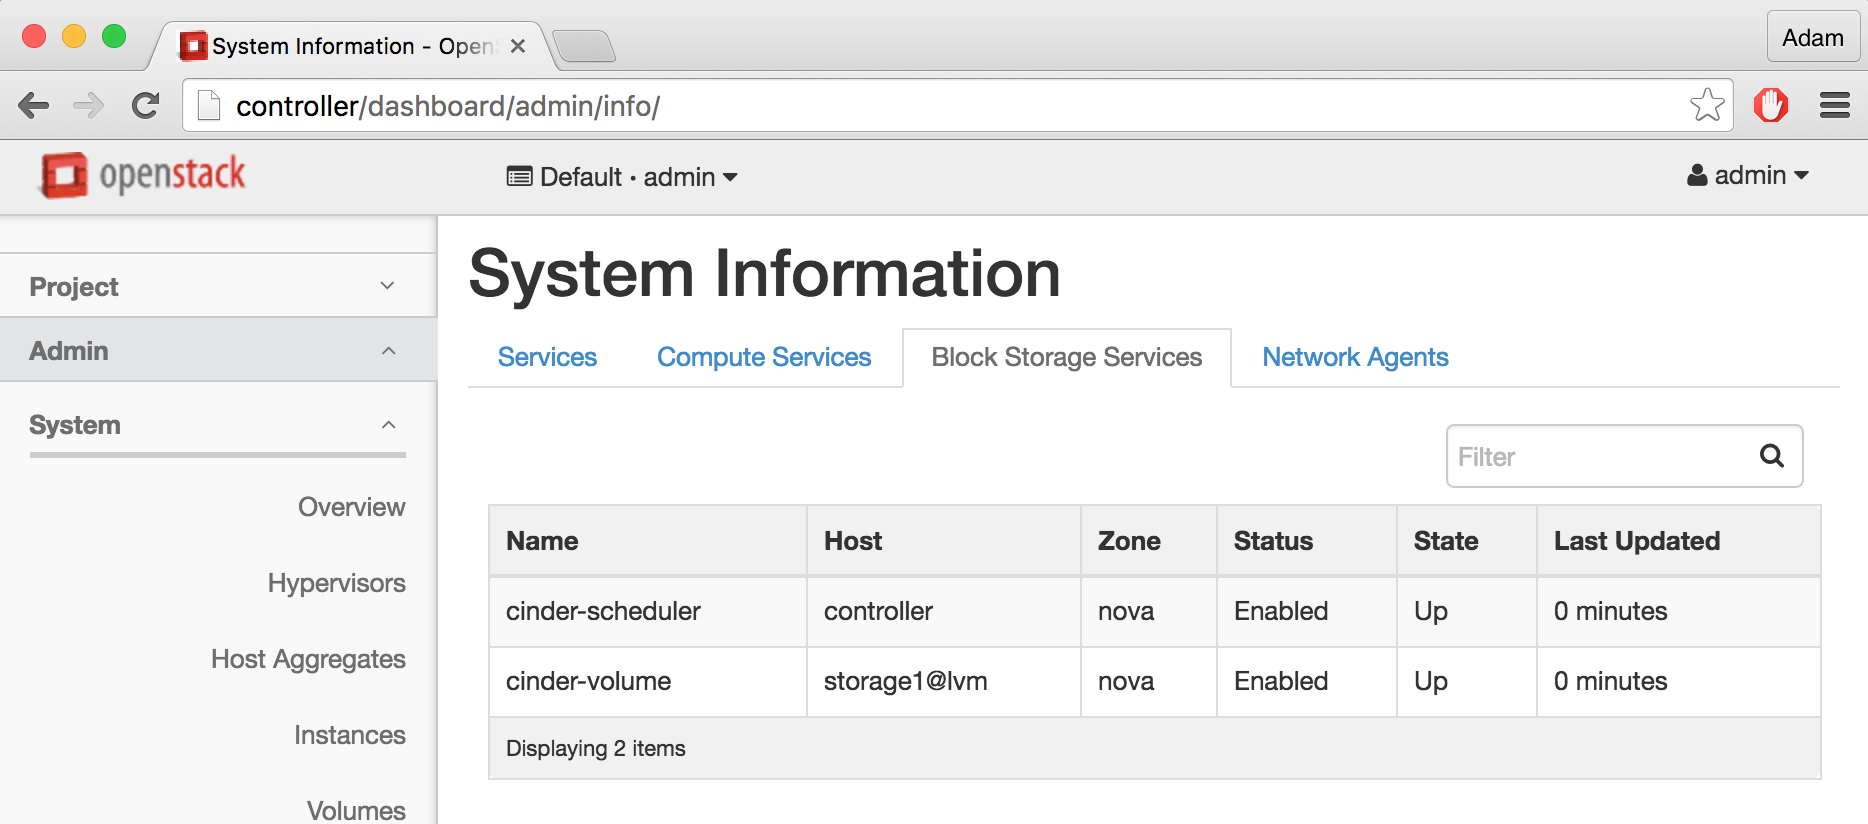
\includegraphics[width=\textwidth]{fig/screenshot_storage.png}
  \caption{The OpenStack Dashboard shows the block storage services running}
  \label{fig:screenshot_storage}
\end{figure}


\begin{figure}[!h]
  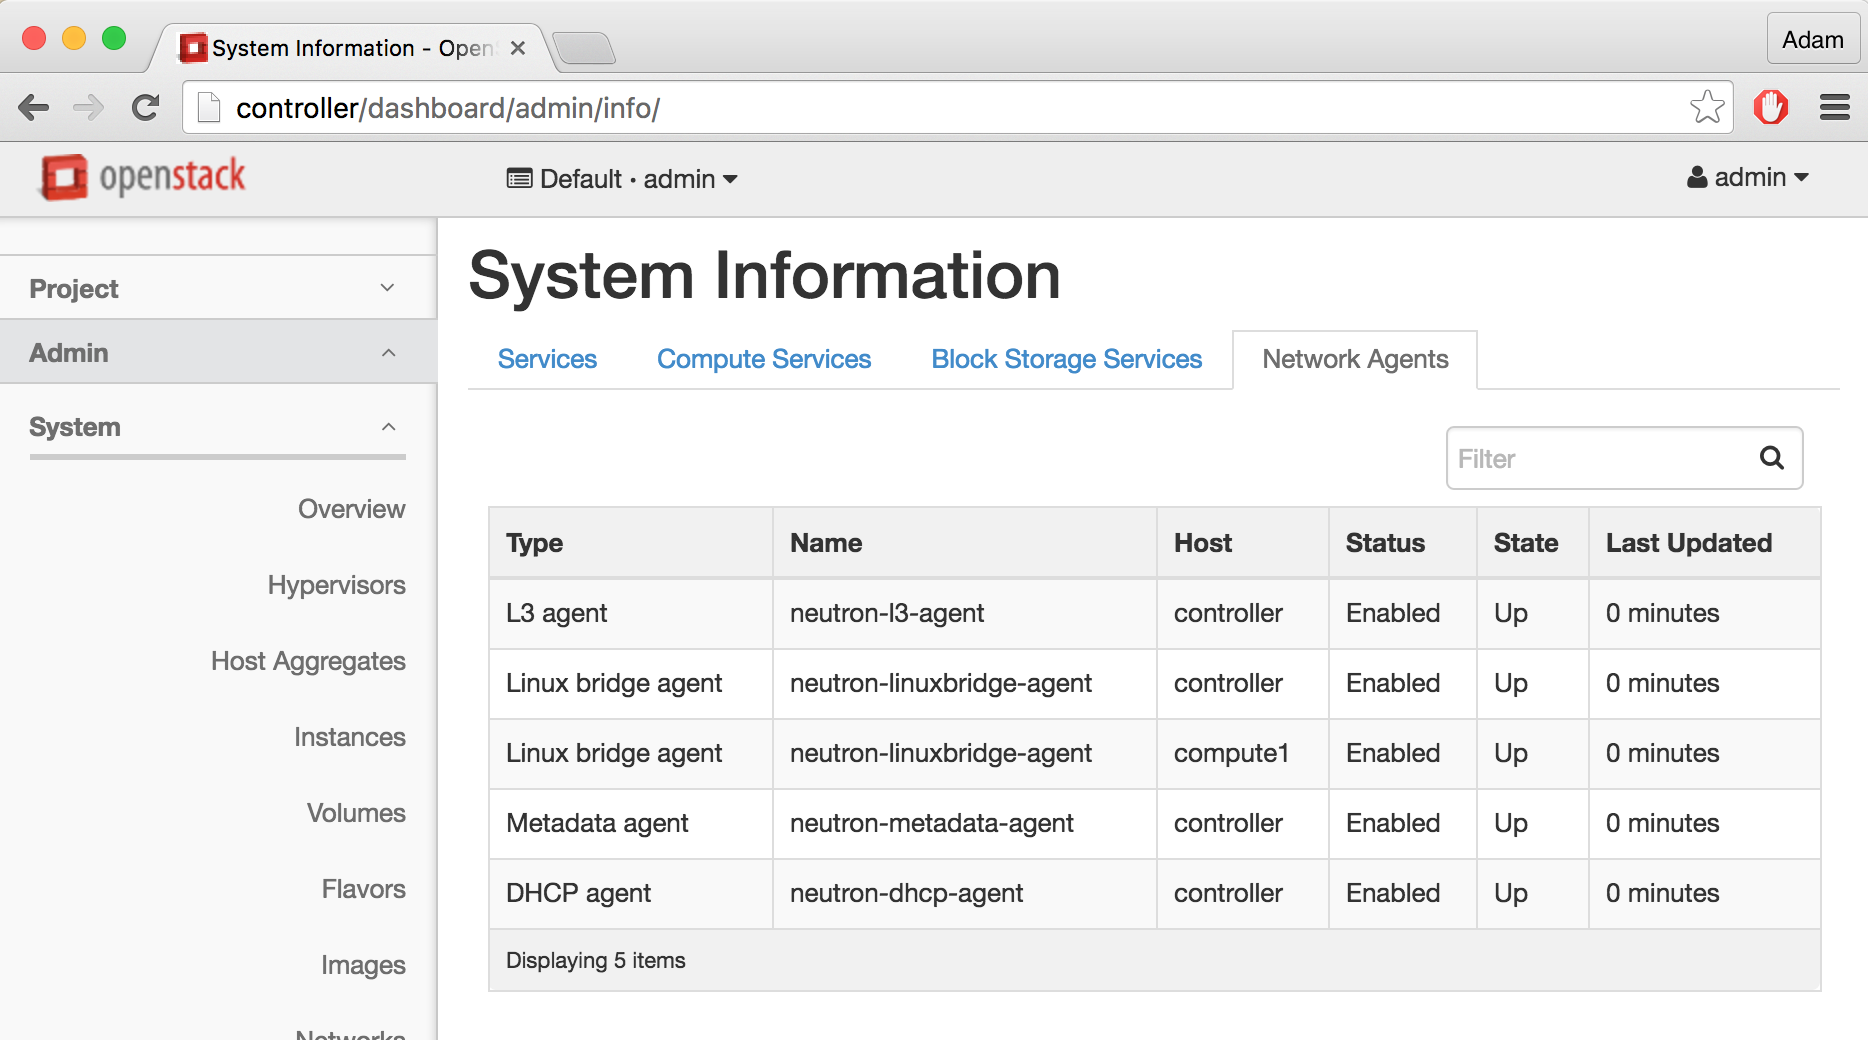
\includegraphics[width=\textwidth]{fig/screenshot_network.png}
  \caption{The OpenStack Dashboard shows the network agents running}
  \label{fig:screenshot_network}
\end{figure}


\subsubsection{Testing the Functionality}

To test the deployment functionality, I have created six virtual machines, two tenant networks, one router, and one provider network. The picture \ref{fig:screenshot} is a screenshot showing the whole environment running in the OpenStadk Dashboard.


\begin{figure}[!h]
  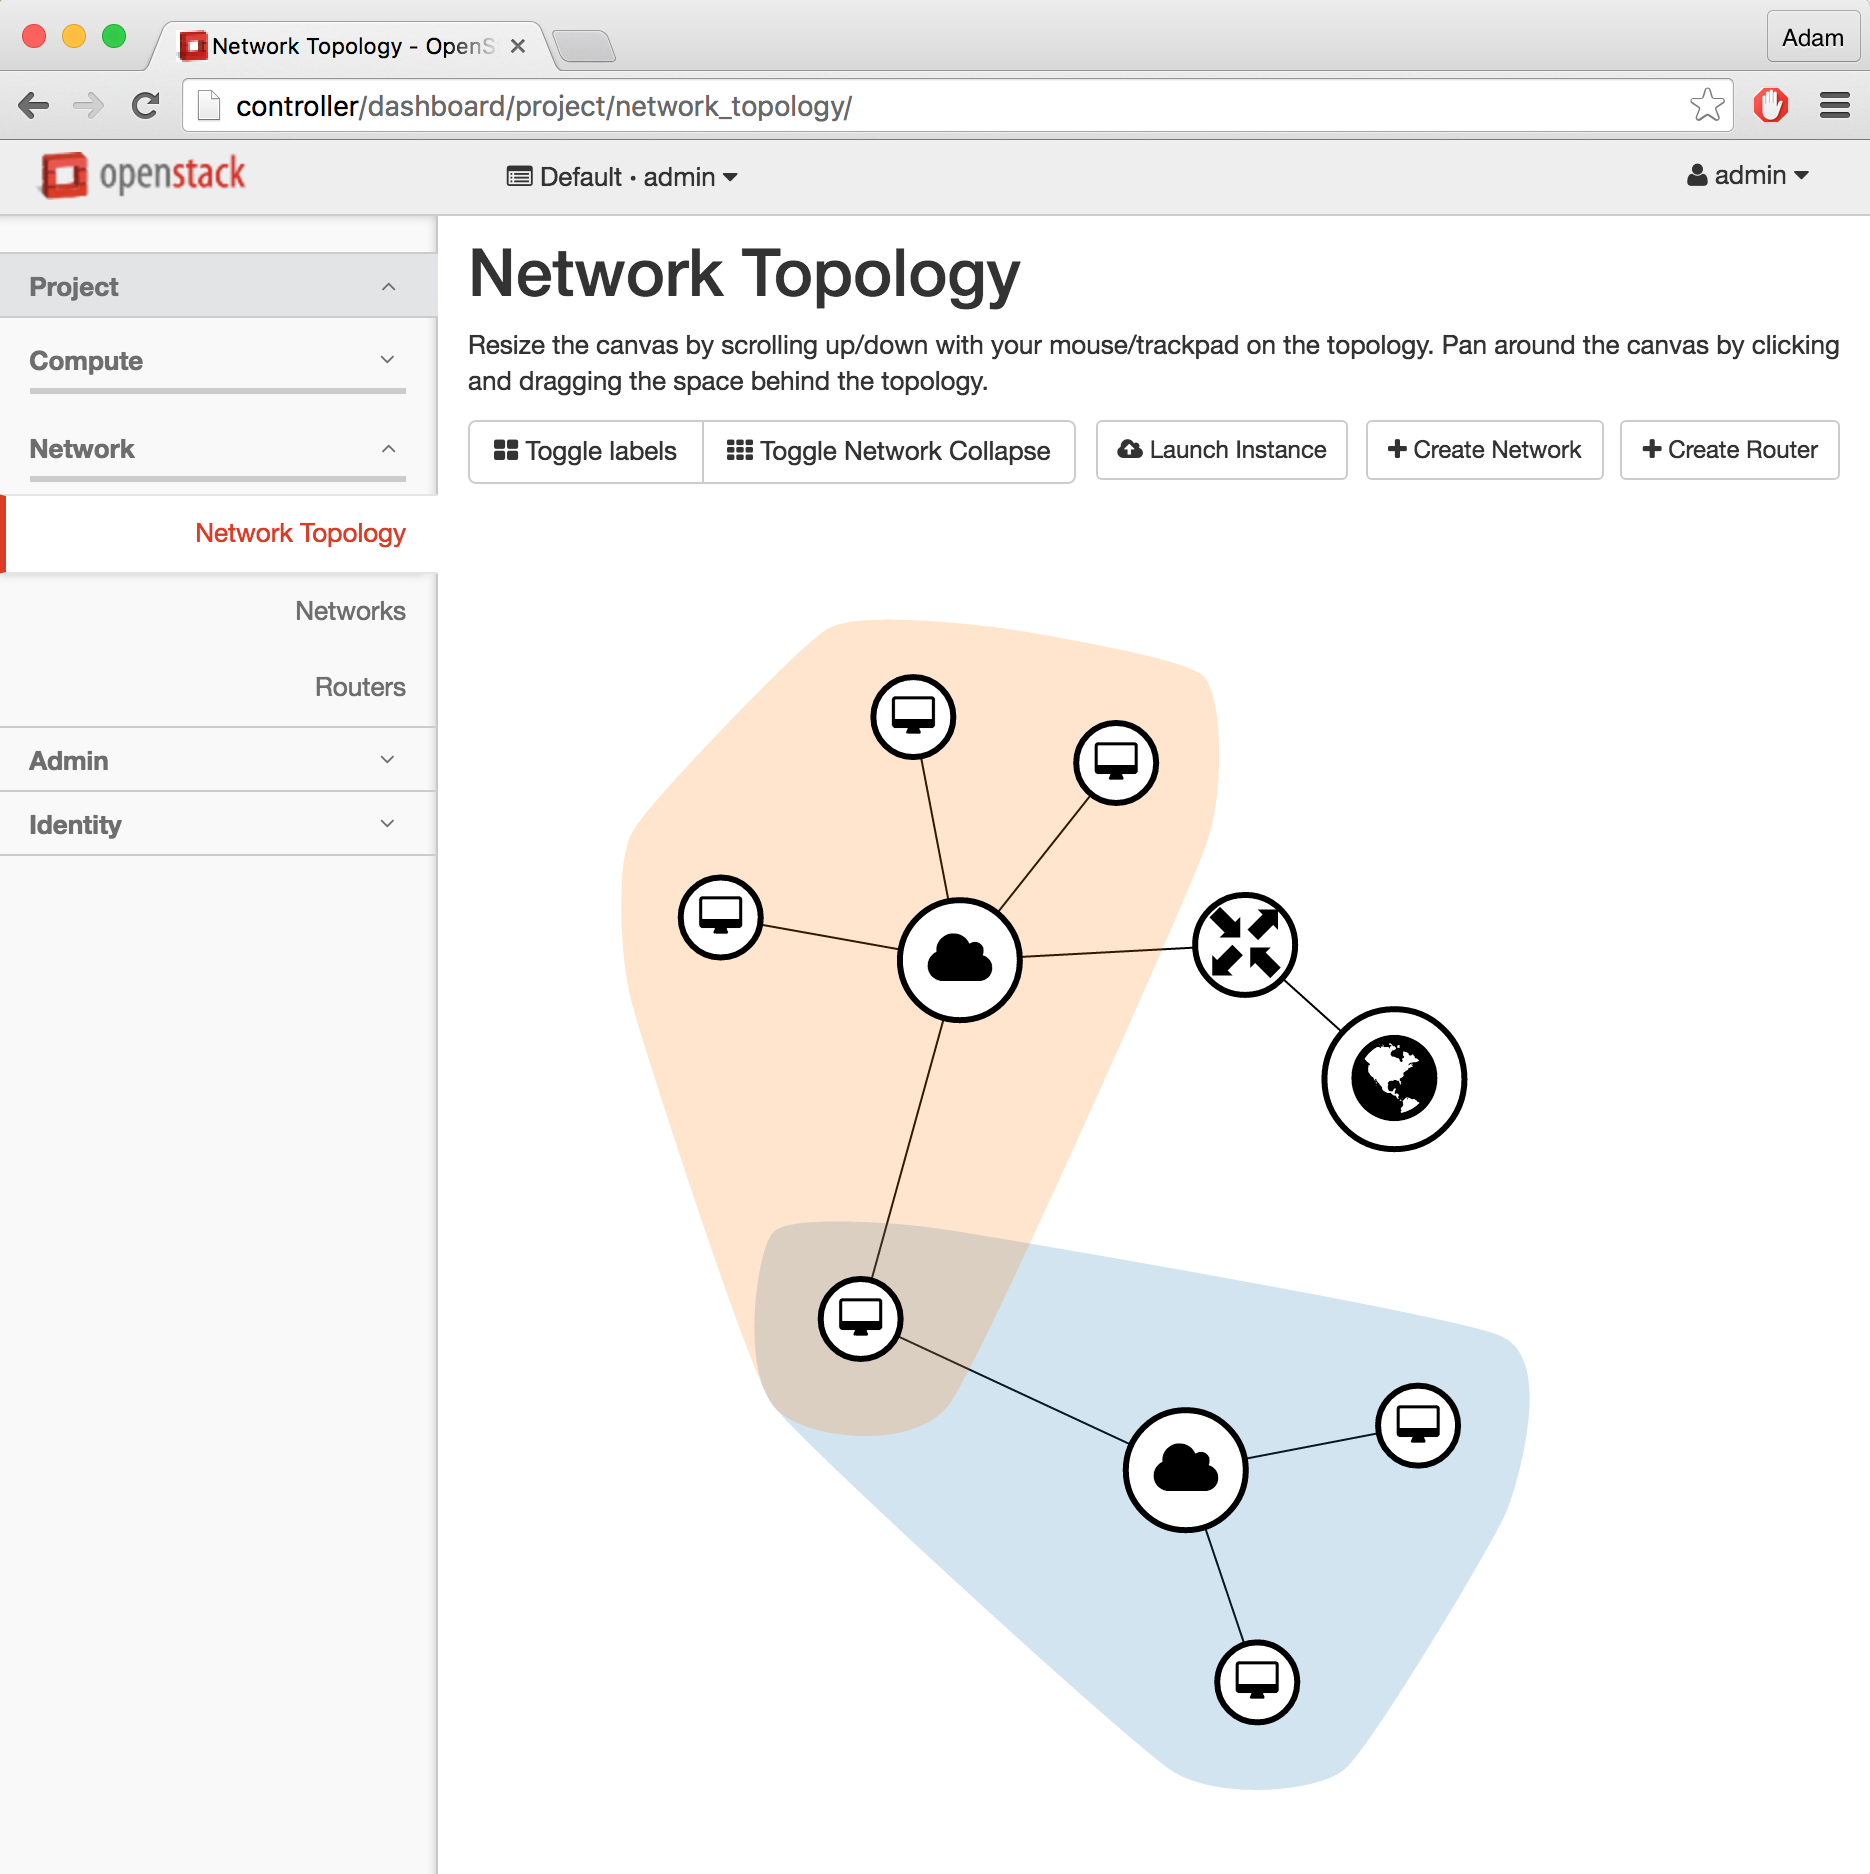
\includegraphics[width=\textwidth]{fig/screenshot.png}
  \caption{The OpenStack Dashboard shows the testing environment}
  \label{fig:screenshot}
\end{figure}
